\documentclass[]{sig-alternate}
%\usepackage{latex8}
%\usepackage{times}
\usepackage{alltt}
\renewcommand{\ttdefault}{txtt}

\usepackage{amsmath}
\usepackage{amssymb}
\usepackage{blindtext}
\usepackage{graphicx}
\usepackage[font=small]{caption,subfig}
\usepackage{placeins}
\usepackage{listings}
\graphicspath{{./fig/}}

\usepackage[usenames]{color}
\usepackage{lipsum}% http://ctan.org/pkg/lipsum
\usepackage{multicol}% http://ctan.org/pkg/multicols
%\pagestyle{empty}
\usepackage{textgreek}

%%to fix indentation of enumerated lists
\let\labelindent\relax
\usepackage{enumitem} 
\usepackage{algorithm} 
\usepackage{algpseudocode}
\usepackage[noadjust]{cite}

\usepackage{multirow}
%%% Spacing Stuff
%\newcommand{\figVspaceBefore}{\vspace{0mm}}
%\newcommand{\figVspaceBetween}{\vspace{0mm}}
%\newcommand{\figVspaceAfter}{\vspace{0mm}}
%\topsep 0in \itemsep 0in        % No extra space in itemized lists

%%% misc commands
\newcommand{\eg}{{\it e.g.}\thinspace}
%\newcommand{\ie}{{\it i.e.}\thinspace}
\newcommand{\ie}{{\it i.e.}\thinspace}
\newcommand{\etc}{{\it etc.}\thinspace}
\newcommand{\etal}{{\it et al.}\thinspace}

\newcommand{\note}[1]{\textcolor{red}{\it NOTE: #1}}
\newcommand{\hilite}[1]{\textcolor{blue}{#1}}
\newcommand{\change}[1]{\textcolor{red}{\textbf{\textit{#1}} }}
%\newcommand{\change}[1]{\hl{#1}}
\newcommand{\squeezelist}{
  \setlength{\topsep}{0pt}
  \setlength{\parskip}{0pt}
  \setlength{\partopsep}{0pt}
  \setlength{\parsep}{0pt}
  \setlength{\itemsep}{0pt}
}
 
%% Spacing Stuff
\newcommand{\figVspaceStart}{\vspace{-2mm}}
\newcommand{\figVspaceBefore}{\vspace{-3mm}}
\newcommand{\figVspaceAfter}{\vspace{-3mm}}
\topsep 0in \itemsep 0in         % No extra space in itemized lists
\setlength{\tabcolsep}{1.5mm}      % squeeze table columns

\hyphenation{micro-arch-itecture}
\hyphenation{micro-arch-itectur-al}
%\renewcommand{\baselinestretch}{0.9}
\lstset{language=Python,captionpos=b,caption={ConfigParser format snippet},label=DescriptiveLabel}

\author{
  Abhilash Dighe\\
  \texttt{adighe@umich.edu} 
  \and
  Nikita Bhutani\\
  \texttt{nbhutani@umich.edu}
  \and
  Pallavi Moghe\\
  \texttt{pallavim@umich.edu} 
  \and
  Vaibhav Gogte\\
  \texttt{vgogte@umich.edu}
}
\title{HOLA: Heuristics for Optimizing Loop Unroll Factors using Machine Learning Algorithm\\\vspace{-4mm}}


\begin{document}


\makeatletter
\def\@copyrightspace{\relax}
\makeatother

%\vspace{4mm}
\maketitle




\begin{abstract}
Compilers rely on efficiency of the intermediate passes to optimize the machine code. Owing to emergence of high performance architectures today, there are many opportunities available to the compiler for optimizing the machine code. We focus on loop unrolling, one such compiler optimization, to extract parallelism and enable better instruction scheduling. Owing to a huge search space in machine code, machine learning algorithms can account for dependencies between several optimization characteristics at once with the same runtime cost. In order to evaluate the effectiveness of machine learning techniques for optimizing compiler passes, we develop heuristics for loop unrolling using random forest algorithm.  We use LLVM Compiler v3.3 to implement and evaluate our heuristics using SPEC 2006 benchmarks. We obtain a speedup of XX percent on our testing set of benchmarks over a baseline LLVM compiler. In addition, even with our limited training set, we obtain performance comparable to the loop unroll pass that is inbuilt in LLVM.
\end{abstract}

\begin{figure*}
  \center
  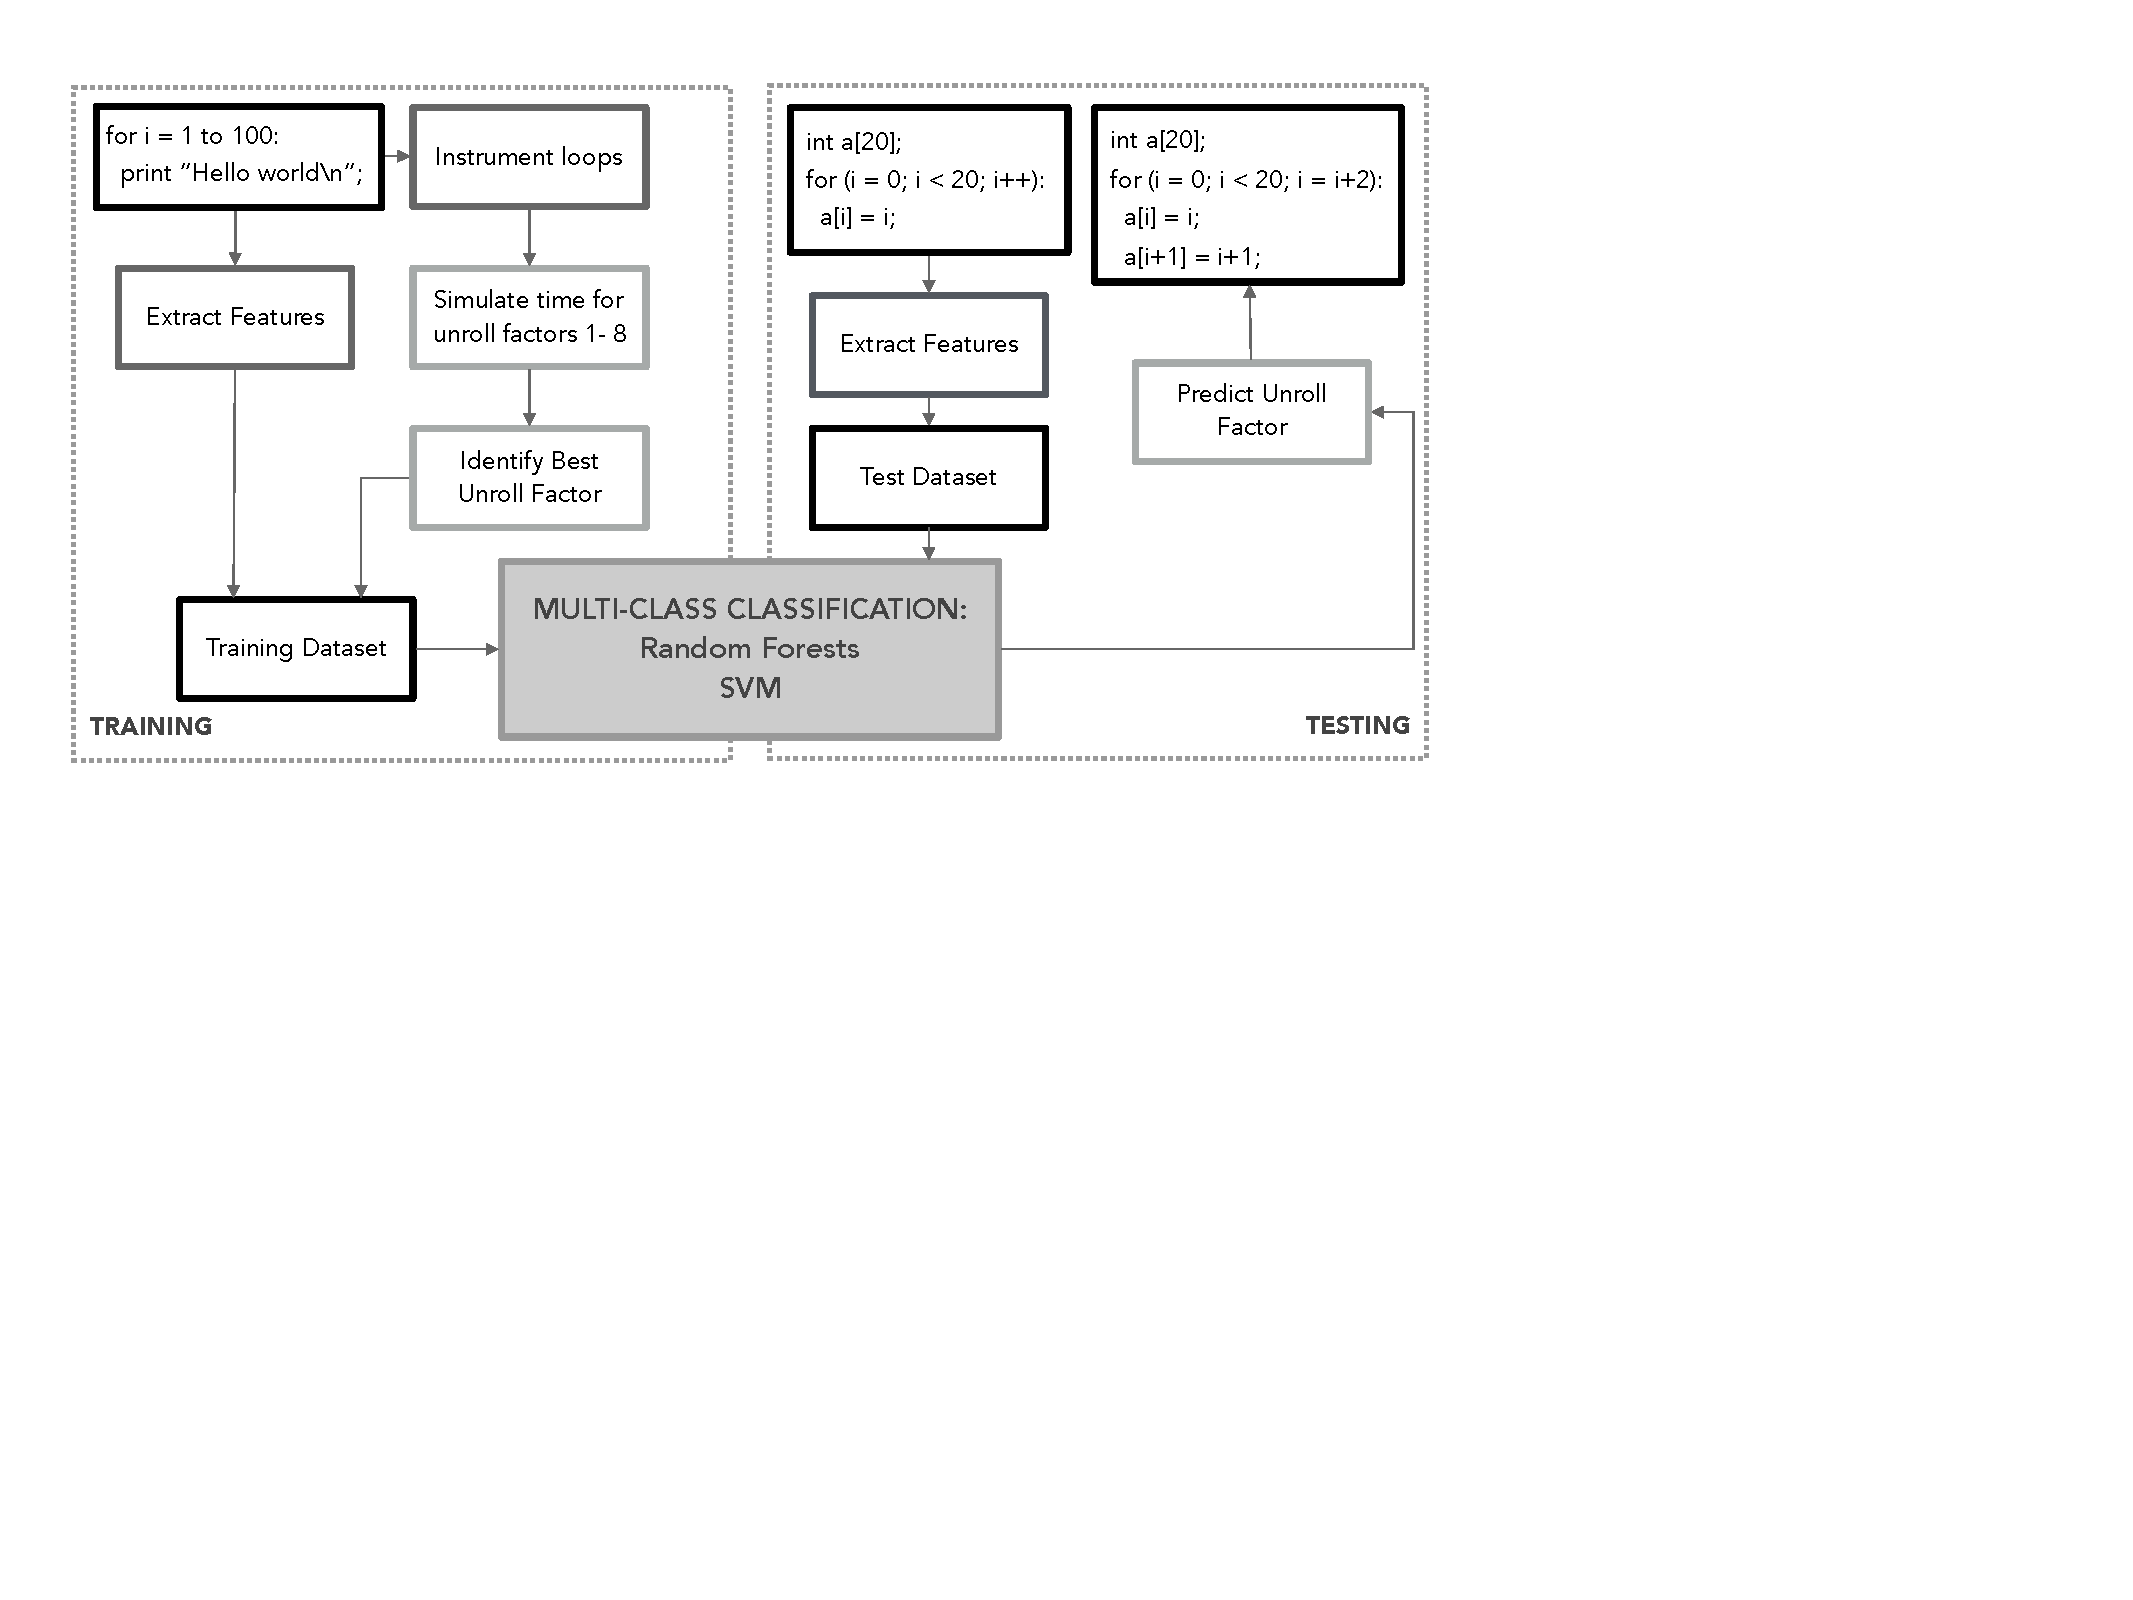
\includegraphics[width=0.90\linewidth]{fig/systemArchitecture.pdf}
  \caption{System Architecture}
  \label{fig:systemArchitechture}
\end{figure*}


\section{Introduction}\label{sec:intro}
Researchers, for generations, have found efficient solutions to optimize machine code generated by a compiler. Multiple traditional optimizations such as loop inlining, loop unrolling, speculative loop invariant code motion, code block ordering, etc. enable vast opportunities to optimize machine code. Majority of these optimizations, exploit parallelism in the machine code so that the instructions can be scheduled efficiently in modern superscalar processors. However, these optimizations are computationally intensive and can often result in degraded performance when done aggressively. As a result, it is important to regulate these optimizations by implementing intelligent heuristics to determine the sections of the code for which the optimizations can be profitable.

Emerging machine learning techniques are known to analyze a huge search space of data and implement intelligent predicting models. These techniques can evaluate multiple decision variables at once and can account for dependencies between several such variables. The goal of our project is to explore a machine learning technique as an efficient alternative to develop heuristics for compiler optimization passes. We use supervised learning technique to obtain these heuristics. Supervised learning techniques train heuristics over labeled data consisting of a vector of heuristics and desired output value. As a case study, we develop heuristics for loop unrolling using the random forest machine learning technique.
Random forest technique works on the principle of decisions trees; it generates multiple decision trees, obtains classification from each of them, and chooses the classification that gets majority of the votes. Unlike decision trees, random forests are not prone to overfitting and hence a better candidate while deploying a heuristic working on a wide variety of data set.

We train a random forest based heuristic on a subset of loops in SPEC 2006 benchmarks. SPEC 2006 benchmarks are used widely by the research community to evaluate performance of both, the compiler optimization and the underlying hardware. We divide a set of applications in SPEC 2006 benchmark in two categories  training set and testing set. We generate a set of features for a loop and the unroll factor that enables the best runtime of that loop over the training set to obtain a labeled dataset. We use this labeled data to train the heuristic and finally deploy it on the testing set for evaluation.

\section{Loop unrolling}\label{sec:unroll}
Loop unrolling is a widely used compiler optimization pass targeting simpler loops in the program. Programs spend a significant duration of their execution time in the loops and hence, it is important to efficiently schedule instructions in a loop to exploit parallelism in them. Due to the iterative nature of the loop, control flow has to branch to the header every time the loop condition is satisfied. These branches are expensive and result in underutilization of hardware optimizations such as superscalar processors, load-store coalescing, cache locality etc. Loop unrolling technique expands the loops several times while reducing the number of iterations and consequently, diminishing the number of branches. The advantages of loop unrolling are several as listed below:

\noindent $\bullet$ Better instruction scheduling as the window to schedule consecutive instruction increases. Hardware can exploit higher ILP.

\noindent $\bullet$ Most loops load and store values to an array of memory locations. Loop unrolling can enable the coalescing of such memory operations in the hardware.

\noindent $\bullet$ Reduction in the number of iterations results in fewer number of branches to the loop header. The hardware can load consecutive instructions in the memory without change in the control flow.

Loop unrolling, however, results in some of the obvious side-effects that can result in degraded performance:

\noindent $\bullet$ A code bloat leading to higher memory pressure.

\noindent $\bullet$ Increased code size and limited hardware register resulting in spilling of variables on the stack. Stack is accessed slower than register resulting in degraded program performance.

\noindent $\bullet$ A loop can exit at multiple places; compiler has to insert complex control flow for early exits from the program.

Aggressive loop unrolling can lead to degraded performance of an application. We develop heuristics to determine the profitable loop candidates for unrolling at the compile time.

\section{Approach and Infrastructure}
\label{sec:Approach}

This section discusses how learning good heuristics for loop unrolling can be modeled as a supervised learning problem. It is followed by a discussion of the infrastructure that was used to perform the experiments. 

\subsection{Supervised Learning}
\label{subsec:SupervisedLearning}
Supervised learning is the machine learning task of inferring a function from \emph{training data}. The training data consist of a set of \emph{training examples}. Each example is a pair  $<\mathbf{x_i}, y_j>$ consisting of an input feature vector, $\mathbf{x_i}$ that contains characteristics of the object under consideration and a desired output label $y_j$. A supervised learning algorithm analyzes the training data and produces an inferred function, which is called a classifier, such that the overall classification error on the training data is minimized. The inferred function should then be able to predict correct output value for any valid input feature vector. 

For the task of loop unrolling, the feature vector captures the characteristics of the loop being unrolled. In our experiments, we used features such as trip call count, number of calls to the loop, number of operations in the loop body, etc. to characterize the loops. Feature vectors are extracted for every candidate for loop unrolling in the set of training benchmarks. For feature extraction, every loop is first assigned a unique identifier. The loops are then canonicalized such that every loop has a preheader and exactly one backedge. A subset of features that are based on profiling information and loop-carried dependencies are then extracted. Features such as trip count, that require require additional compiler optimizations like promoting memory references to register references, analyzing scalar expressions in loops etc. are extracted separately, so that they don't affect the statistics for other features. Figure~\ref{fig:features} summarizes the features used to train the classifier in this experiment.

\begin{figure}
  \center
  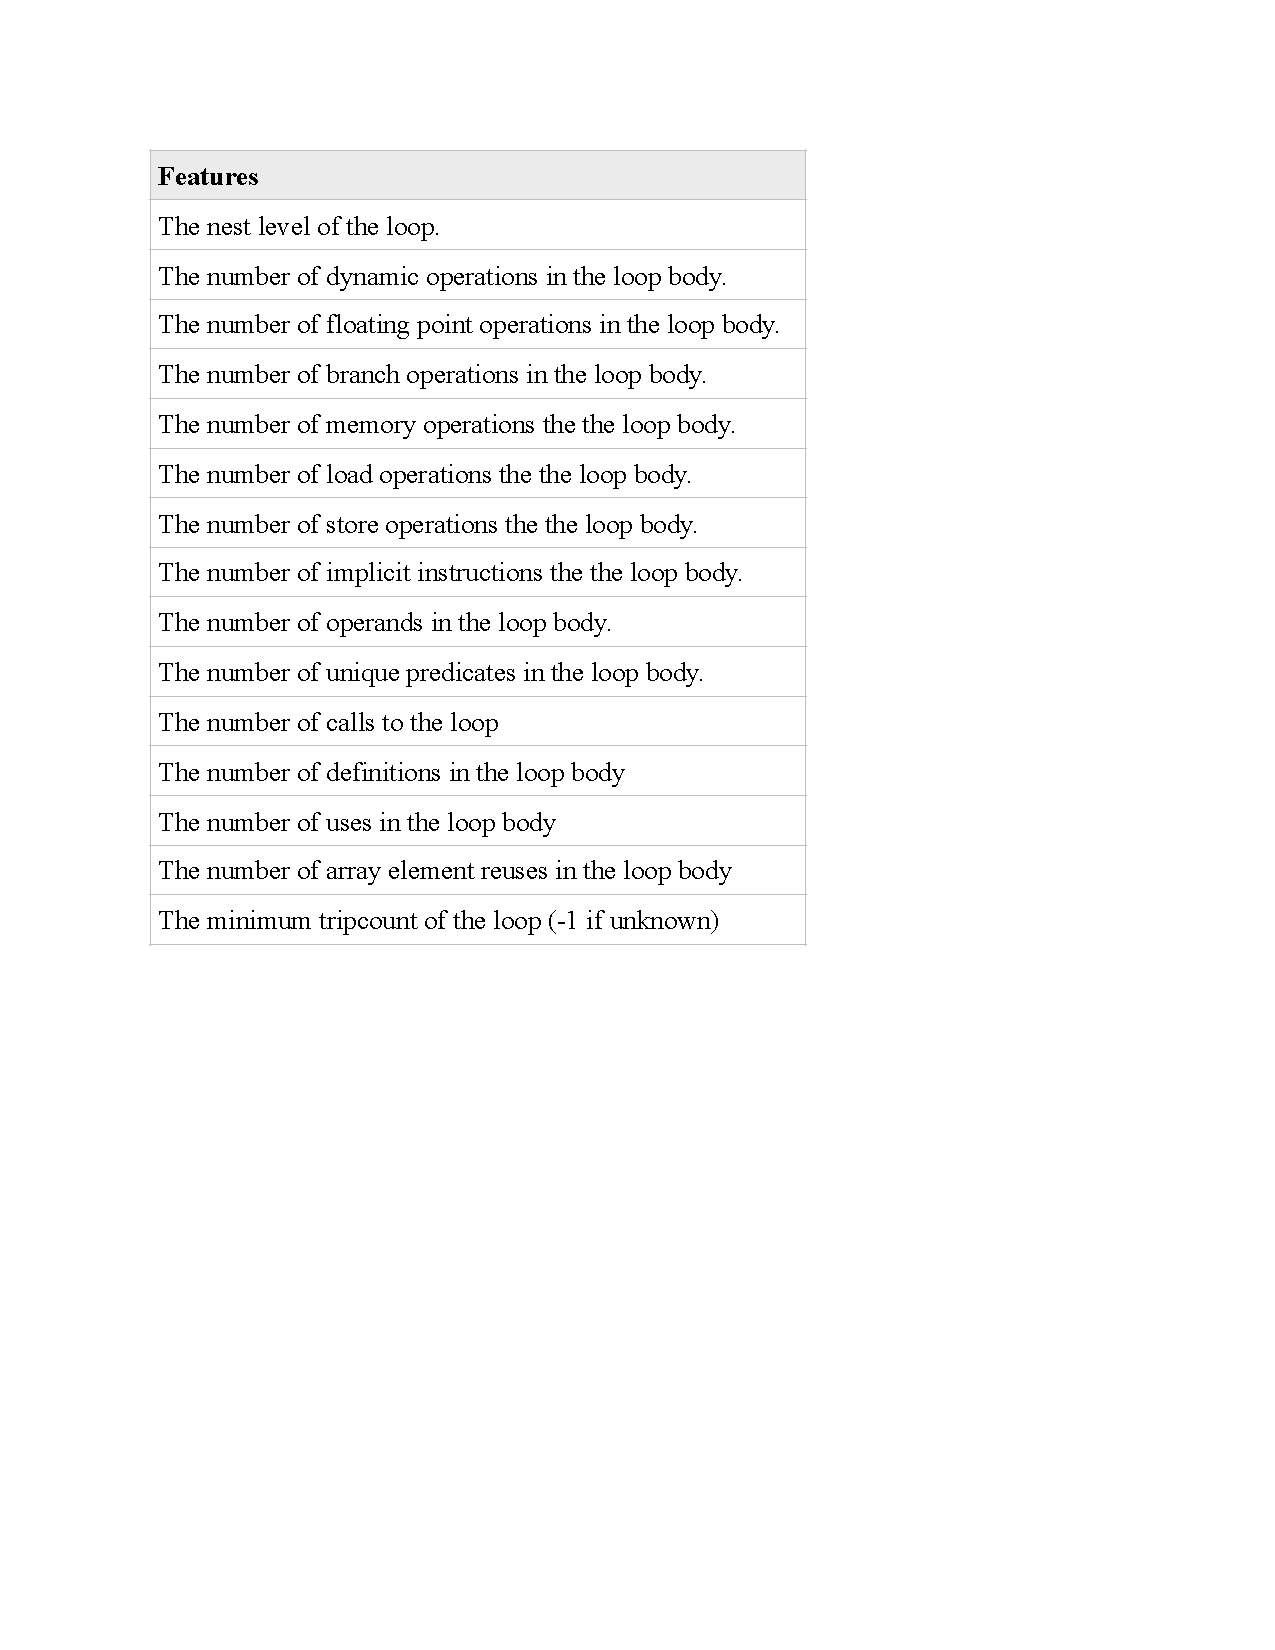
\includegraphics[width=0.90\linewidth]{fig/features.pdf}
  \caption{Features used for the classification task}
  \label{fig:features}
\end{figure}

For the training dataset, we also extract label for each candidate loop in our train benchmark suite. The label for a loop indicates the best unrolling factor for the loop. In this study, the unroll factor (1,2,..8) yielding the best performance for the loop is used as the label for the loop. Thus, each example in the training set corresponds to a feature vector indicating loop characteristics, and a label indicating the best unroll factor derived empirically. The classifier then learns how to best map these loop characteristics, $\mathbf{x_i}$, to their corresponding unroll factor $y_j$. Features for loops in the test benchmark suite are extracted similarly, but since extracting labels is expensive, no labels are extracted for the test benchmark suite. Training the classifier is offline; this approach incurs no overhead at run-time. 

\subsection{Compiler and Platform}
\label{subsec:CompilerPlatform}

We used LLVM (version 3.3) that provides a modern source- and target-independent optimizer, along with code generation support for many popular CPUs. The modules to extract features and labels for the loops along with the module to unroll the loop were written using LLVM. LLVM was selected as it is easy to use and integrate various analysis and transformation passes for feature extraction, label extraction and loop unrolling.  The experiments in this paper were performed on 2.2 GHz Intel Xeon 64-bit 12 core server with 32KB L1 cache, 256KB L2 cache and 16MB L3 cache. For all our experiments all optimizations except for loop-simplify were disabled unless required by another analysis or transform pass. 

\subsection{Loop Instrumentation}
\label{subsec:LoopInstrumentation}

In order to collect labels for the loops in the train benchmark suite, the loops must be instrumented. We evaluated three approaches to unroll loops. First, if the profiling is done at program level, all different combinations of unroll factors for the loops in the program must be tried to identify the combination yielding the best performance. Owing to combinatorial considerations, this solution is computationally intractable. Second, the computational intractability in loop level profiling can be handled by analyzing the loops from innermost to outermost such that optimal unroll factor for the innermost loop is first identified. Subsequent loops are analyzed after the innermost loop is unrolled by the optimal unroll factor. However, this approach is expensive because the program being analyzed must be executed \emph{no. of loops * no. of unroll factor} times. Also, to implement such a system is not straightforward. We instead used \emph{loop level profiling} wherein each loop is analyzed in independently of other loops. The central idea is to instrument each loop so the execution time for each loop can be determined, and then unroll every loop in the program by an unroll factor (1,2...8). Optimal unroll factors for each loop are then determined based on their performance. Although the instrumentation at loop level is a bit intrusive, the program has to be executed only once for each unroll factor, reducing the time/cost of generating the training dataset.

We invested much engineering effort minimizing the impact that the instrumentation code has on the execution of the program. Instead of relying on a third-party instrumentation library, we wrote our own instrumentation library consisting of two functions namely, \emph{startTimer} and \emph{endTimer} . Our loop instrumentor inserts an instruction that calls the start timer function at the start of the loop. An instruction to call the end timer function is inserted at each exit of the loop. In our preliminary experiments, we printed the running time of each loop at loop exit. But this instrumentation technique was abandoned due to high file I/O overhead incurred at each loop exit. This problem was aggravated for inner loops that are executed more frequently than outer loops. To reduce this overhead, at all exit points in the program a call is made to our instrumentation library to print the cumulative running time of each loop in the program. Figure~\ref{fig:instrumentation} shows how the calls to the library are inserted at the start and exits of the loop.

We realize that we cannot possibly measure loop runtimes without affecting the execution in some way. However, since the instrumentation will affect loops with all unroll factors similarly, it does not affect the choice of optimal unroll factor for a loop. 

\begin{figure}
  \center
  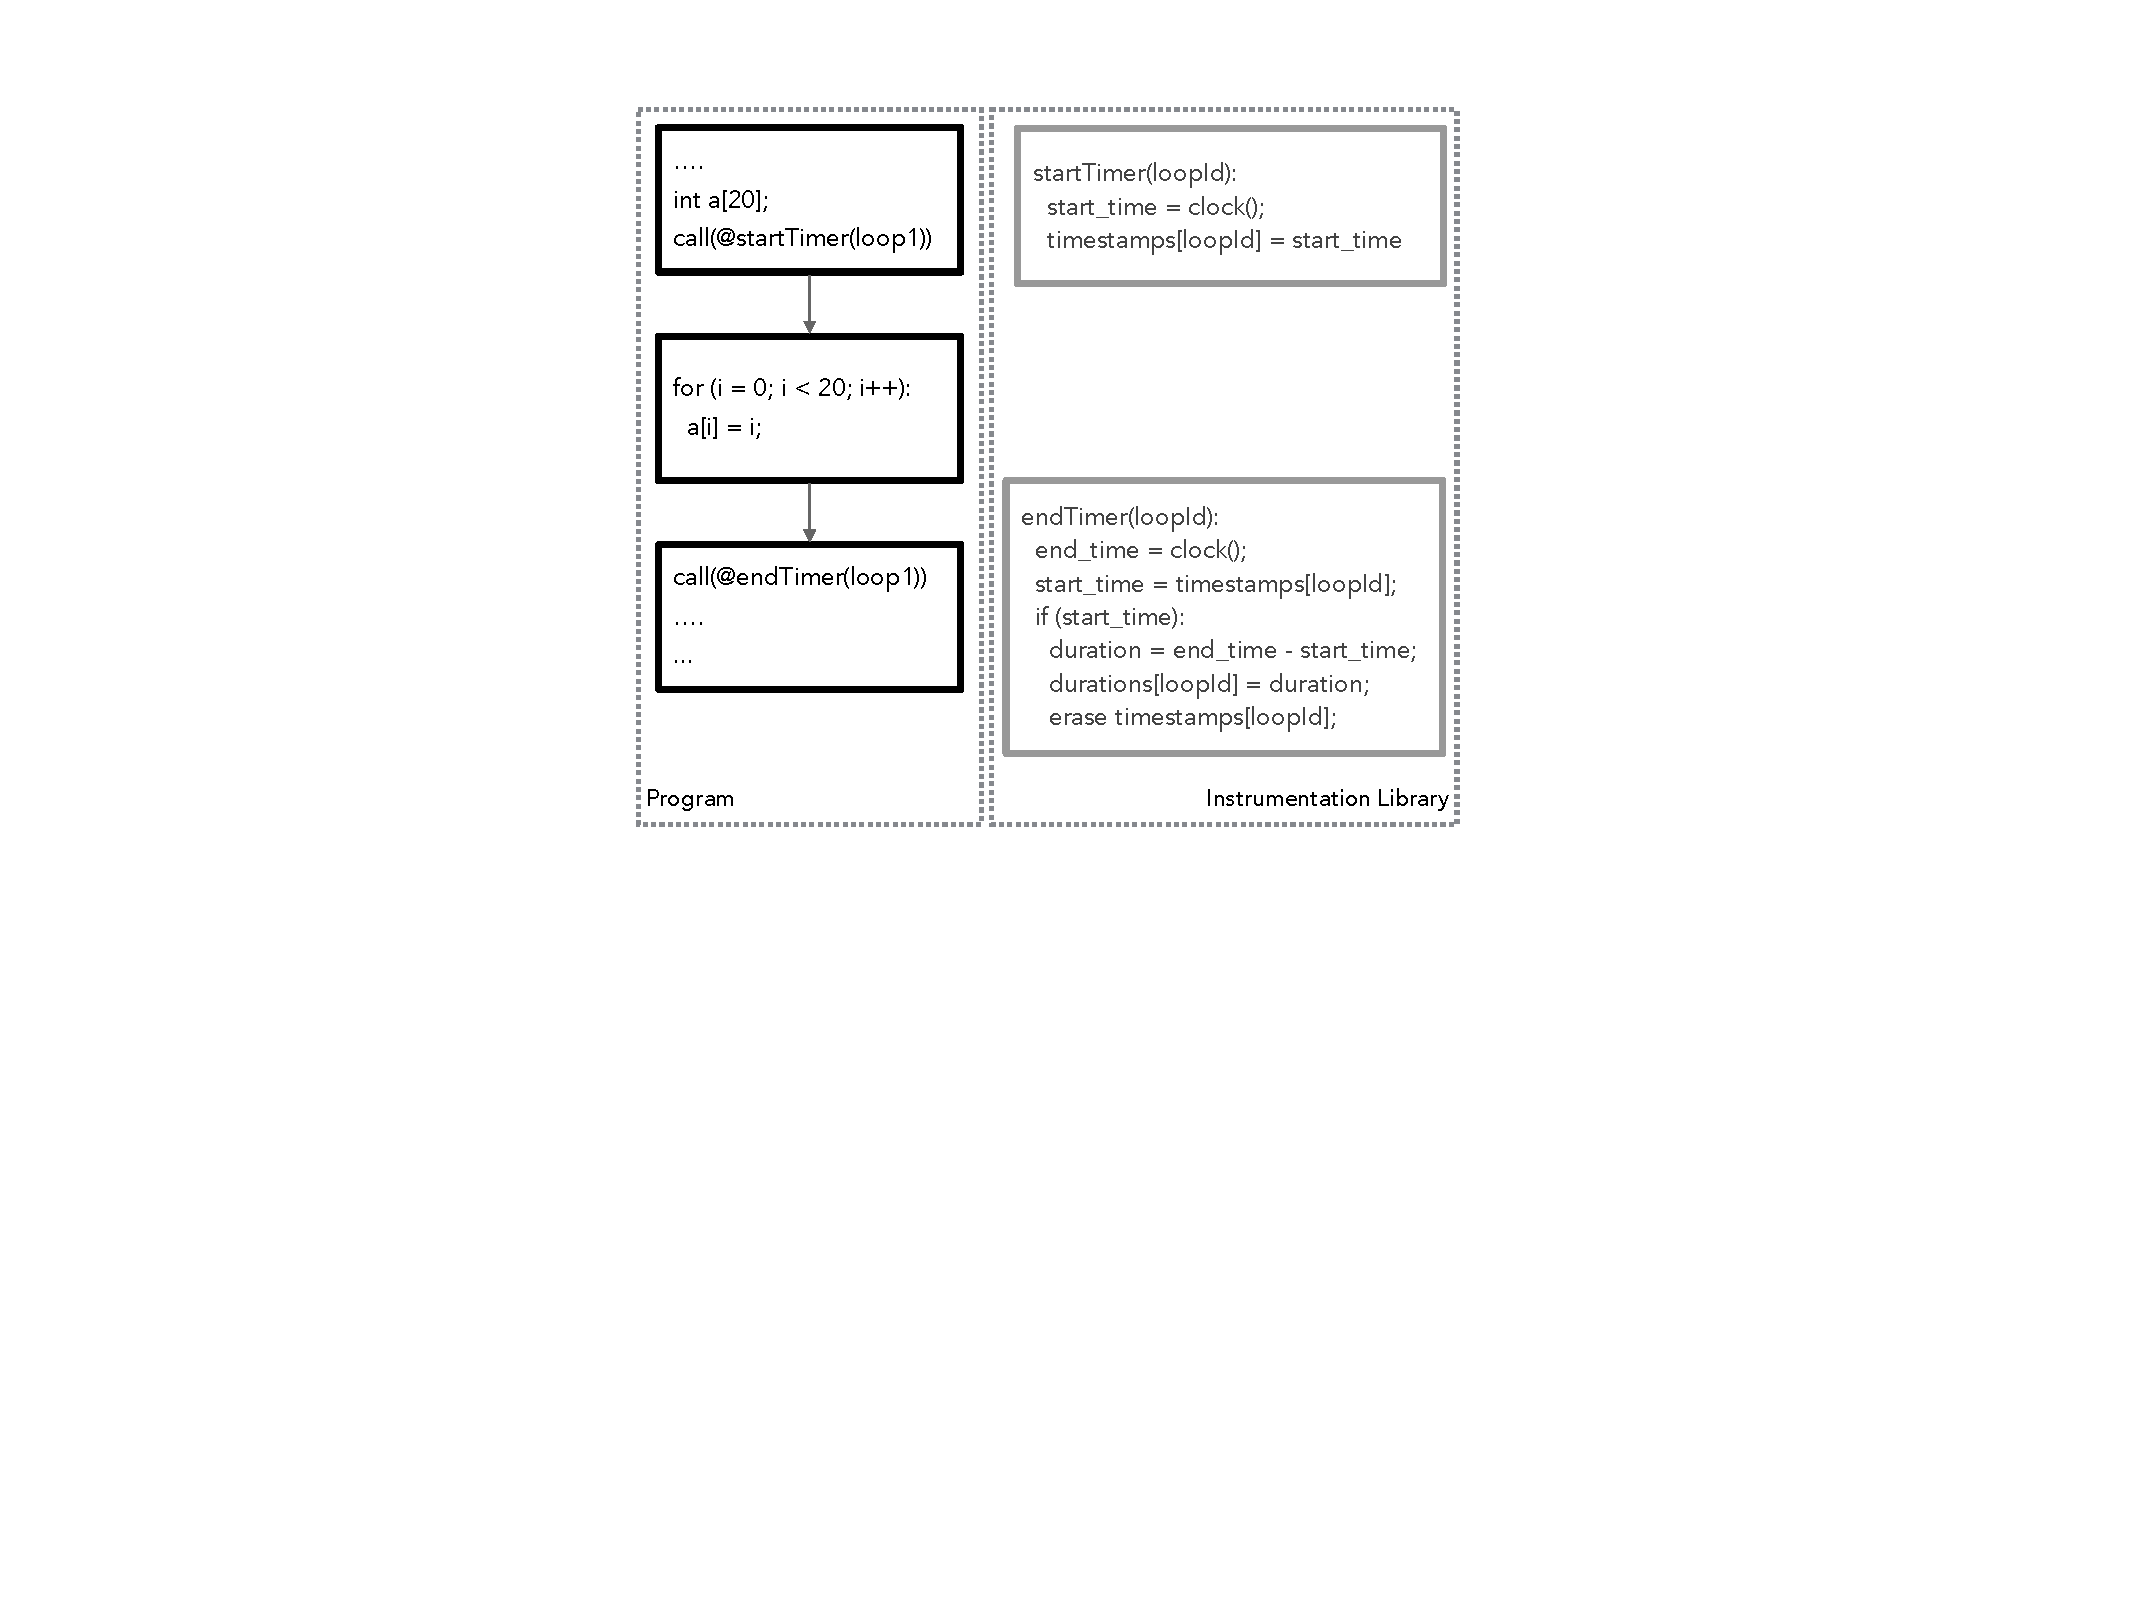
\includegraphics[width=0.90\linewidth]{fig/instrumentation.pdf}
  \caption{Instrumentation of loops}
  \label{fig:instrumentation}
\end{figure}

\subsection{Data collection}
\label{subsec:DataCollection}


To extract features for loops in the train benchmarks, we run each benchmark through a series of passes that assign a unique label to the loop, canonicalize the loop, profile the edges in the loop, extract profile-based features and extract trip count of the loop. The benchmark is then instrumented and simulation times are found for all unroll factors up to eight; an unroll factor of one corresponds to leaving the loop intact (rolled). For each loop the optimal unroll factor is determined based on the runtime for each unroll factor. Figure 1. shows the system architecture of HOLA. Once the training data is collected, a classifier is trained to learn the mapping from loop characteristics to optimal unroll factor. A histogram of the different optimal unroll factor labels in our traning set is shown in Figure~\ref{fig:trainingHistogram}. The trained classifier is then used to predict best unroll factor for the loops in the test benchmark suite based on their features extracted the same way as the features for loop in train benchmark suite. The predicted optimal unroll factors for each loop in the test benchmark suite are then applied to the corresponding loops. The test benchmarks are then compiled and executed to assess improvement in performance. 


\begin{figure}
  \center
  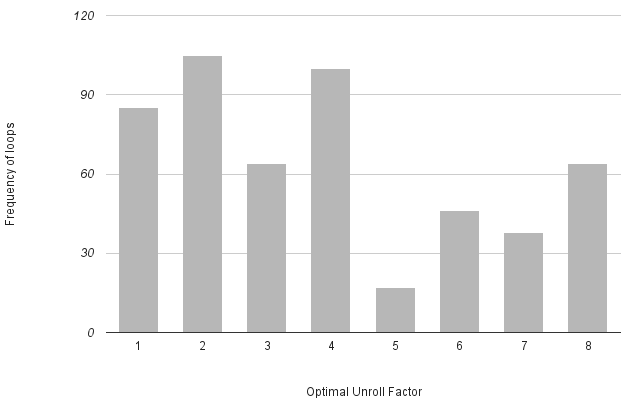
\includegraphics[width=0.90\linewidth]{fig/histogram.png}
  \caption{Training Labels Histogram}
  \label{fig:trainingHistogram}
\end{figure}

\section{Multi-class Classification}
\label{sec:Multi-classClassification}

Multi-class classification is a supervised machine learning problem where the number of different class values is greater than 2. Many binary classifiers can be easily extended to the multi-class domain while some require combining multiple binary classifiers. In this section, we take a look at the different multi-class classification techniques we tried out and their properties. 

\subsection{Logistic Regression}
\label{subsec:LogisticRegression}

Logistic Regression is a commonly used linear model for classification. It measures the relationship between the dependent variable and one or more independent variables by estimating probabilities using a logistic function. It generates a weight vector for the indepdent variables which can be used to predict the dependent variable for the new unseen samples. Being a binary classification problem it isn't directly extendable to the multi-class setting and uses methods such as one-vs-all and one-vs-one for combining multiple binary classifiers into a multi-class classifier. 

\subsection{SVM}
\label{subsec:SVM}

Support Vector Machine is a powerful supervised classification technique which can perform linear as well as non-linear classification using the kernel trick where they map the features into a high dimensional space. The SVM model involves storing multiple data points as representatives of the classes so that the gap between the two classes is as wide as possible. When used for multi-class problems it uses techniques similar to logistic regression. 

\subsection{Neural Network}
\label{subsec:NeuralNetwork}

Neural Network is a machine learning tool inspired by the way neurons interact and learn in the nervous system. It involves learning the weights of the connections in a network of nodes arranged in multiple layers. There is an input layer which has neurons equal to the number of features to train on and an output layer which has a neuron for every possible class output. The network uses the backpropogation algorithm to learn the various weights given labeled training data. 

\subsection{Random Forest}
\label{subsec:RandomForest}

Random Forest is an ensemble method which works by generating N random subsets on the training data in terms of samples and features and constructing a separate decision tree for each subset. It uses only a subset of all the features available which along with the variable datasets help avoid overfitting. For every new unseen data sample, it runs the sample through all the generated decision trees and takes a vote to decide the predicted class. A random forest can also be easily extended to multi-class domain as it can assign any label to leaf nodes. 

\section{Experiments with Classification Algorithms}
\label{sec:ExperimentsClassification}

As mentioned in the previous section, we tried 4 different machine learning algorithms to predict the optimal unroll factors. We needed an experimental setup to to evaluate the average performance of the various machine learning algorithms. In this section we go over the details of the pipeline we used to assess the goodness of each of the methods, how we implemented them and the results of our experiments. 

\subsection{Machine Learning Pipeline}
\label{subsec:MachineLearningPipeline}

We used a standard pipeline shown in Figure~\ref{fig:mlPipeline} for experimenting and evaluating our classification algorithms. Prior to starting the pipeline we gather the features and the optimal unroll factors from all the benchmarks in the training set. We then split the training set into a dev set and a holdout set. Often, classification algorithms need the programmers to set values for certain model parameters such as the regularization parameter in the case of SVM or network structure in the case of Neural Networks. It is imperative to find the optimal values for these parameters to get the most out of the classifier. To find the best model parameters, we first create a grid of possible parameters and then for every candidate parameter, we use K-fold cross-validation to obtain an estimate of its accuracy. K-fold cross-validation involves initially splitting the data into K mutually exclusive and equally sized chunks. Each of the chunks is then kept aside as testing set while the remanining chunks are combined to form the training set. The average of the accuracy achieved over the K-folds is taken as a valid estimate of the goodness of the candidate parameter. The grid search along with K-Fold Cross-Validation is done to decide the best model parameter on the dev set and then the entire dev set is fed into the classifier as training data and the best model parameters are obtained. This best classifier is then tested on the holdout set that its not seen before which gives us a measure of the accuracy of the classification technique on the given labelled training data. This division into the dev and holdout sets is repeated multiple times to avoid wrong estimates due to bad splits. The average of the final accuracies obtained at each iteration is considered as a true estimate of the performance of the particular classification technique on that dataset. 

This final classifier is designed using the entire training set as a dev set with grid search and K-fold cross-validation to find the best model parameters using which the entire training set is fed to the classifier for learning. The features obtained from the test benchmarks are then run through the final classifier to get the predicted unroll factors for each of the loops. 

\begin{figure*}
  \center
  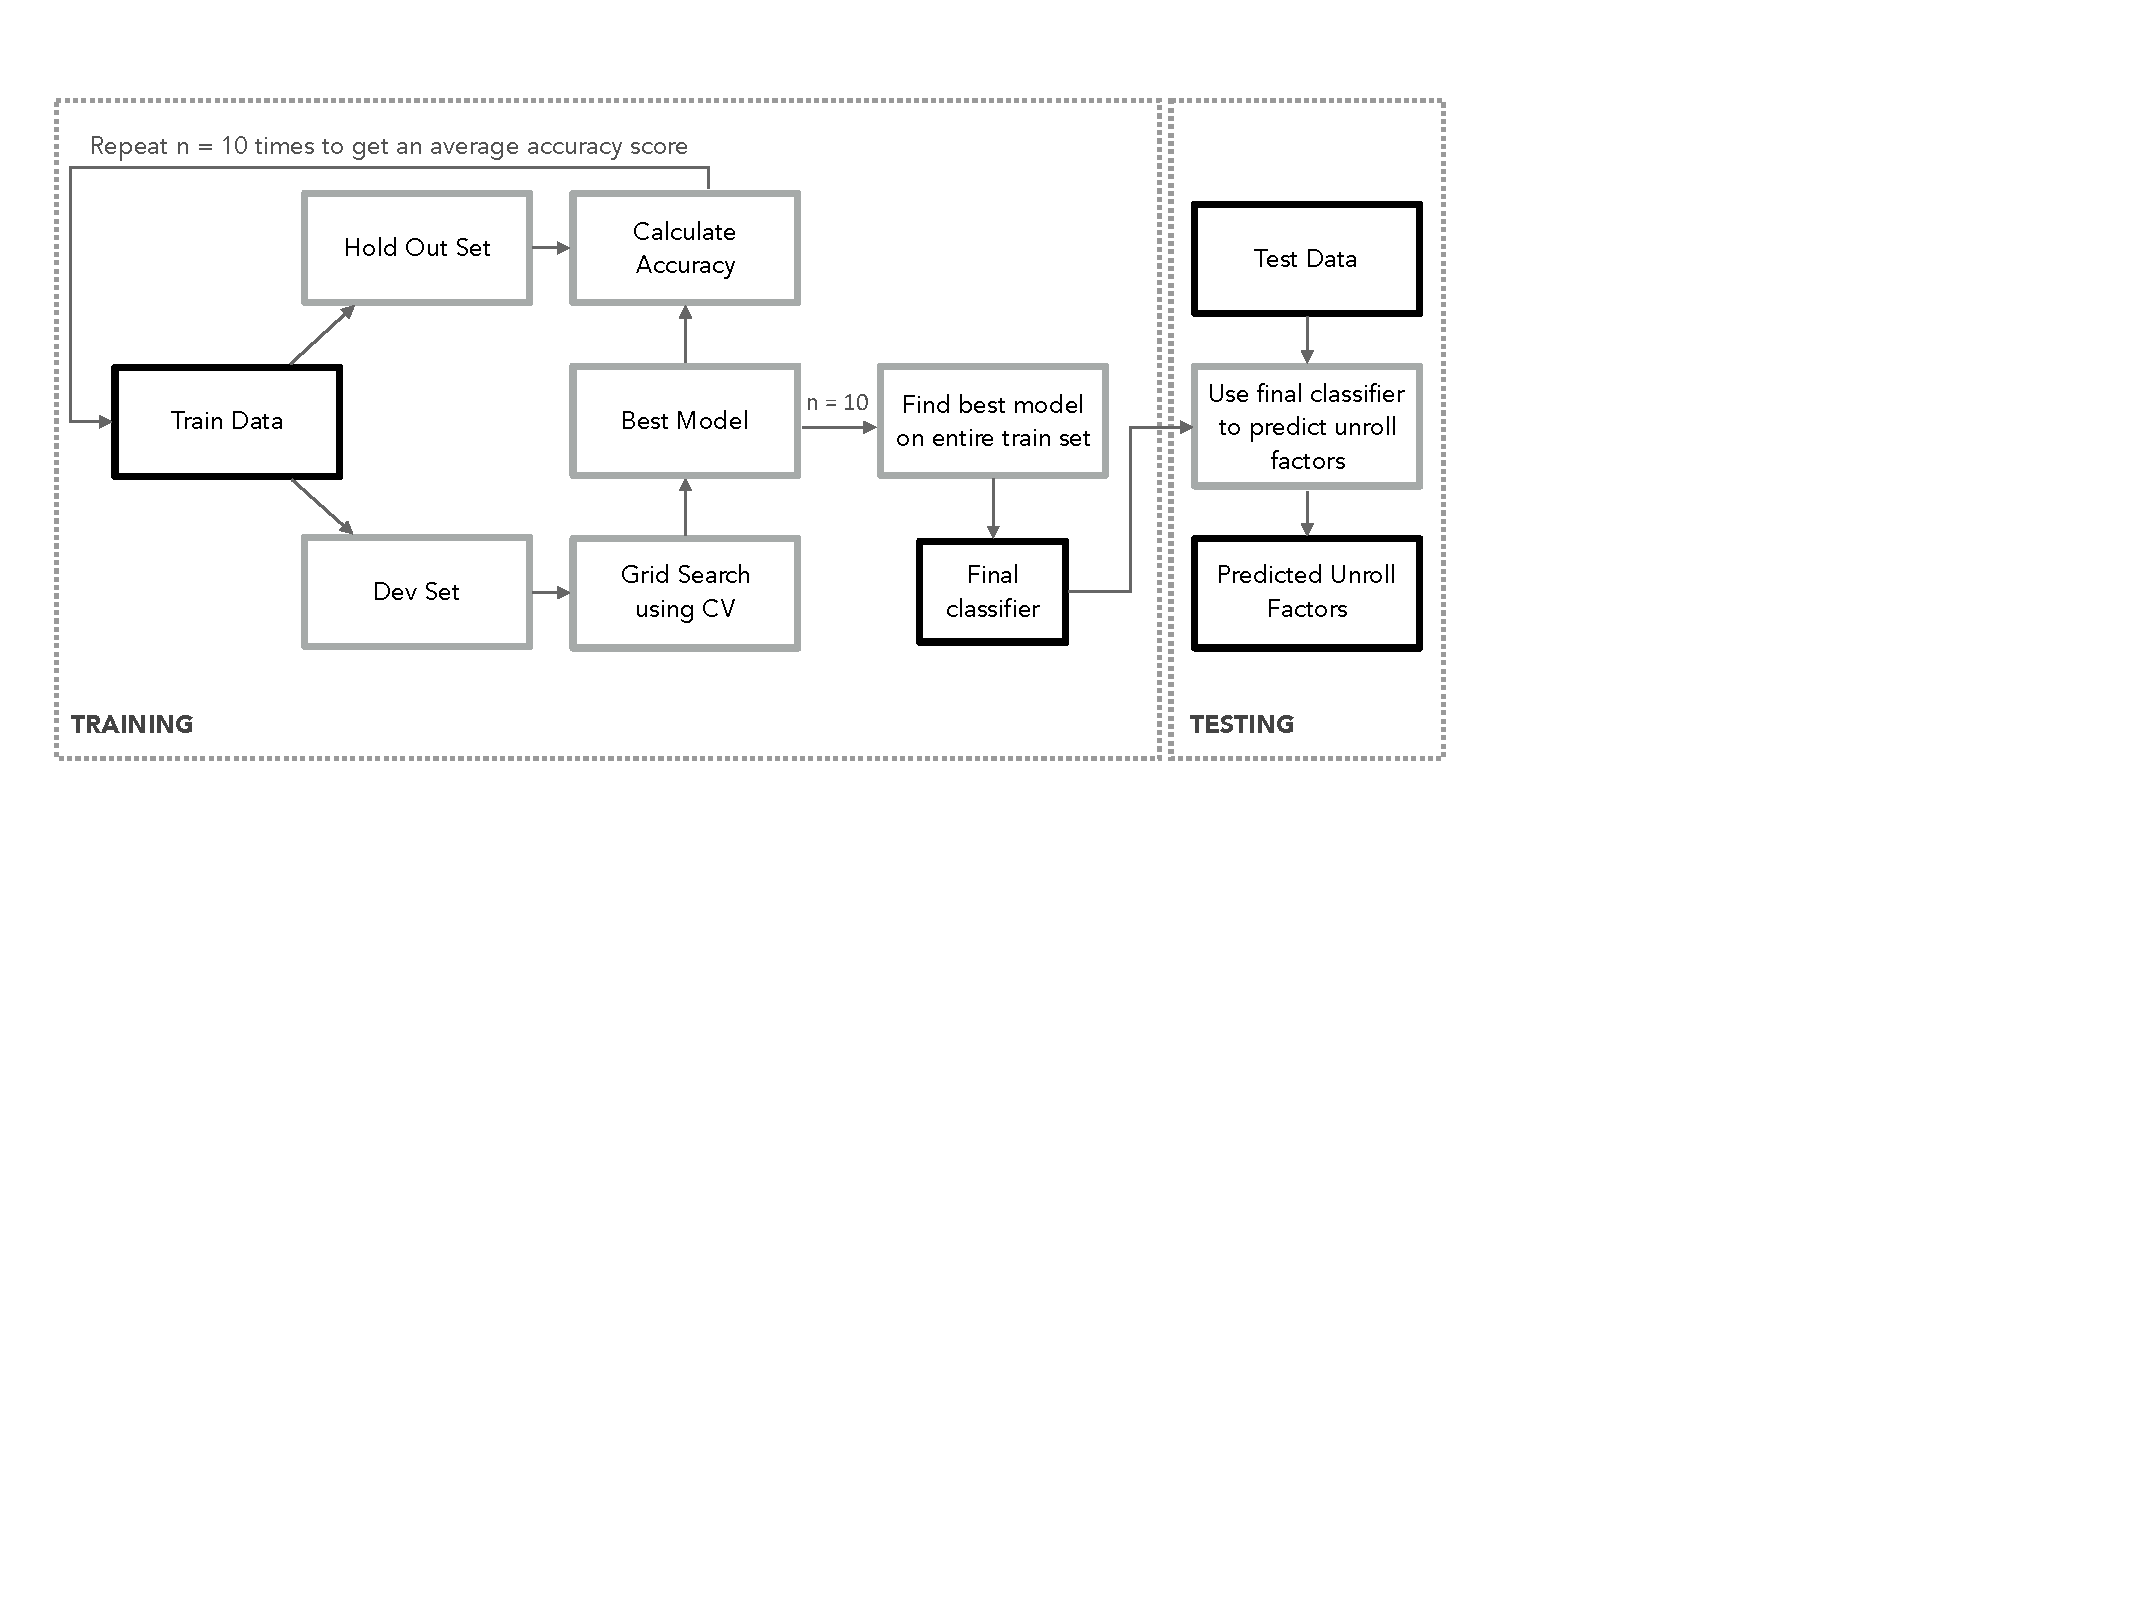
\includegraphics[width=0.9\linewidth]{fig/mlPipeline.pdf}
  \caption{Machine Learning Pipeline.}
  \label{fig:mlPipeline}
\end{figure*}


\subsection{Implementation Details}
\label{subsec:ImplementationDetails}

The Logistic Regression, SVM and Random Forest Classifiers were implemented using the \emph{scikit-learn} module in Python. The module additionally provides implementations of grid search and cross-validation which makes creating the pipeline a bit easier. Neural Networks were implemented using \emph{skflow} which is a \emph{scikit-learn} like interface into Google's recently released Tensorflow library for deep neural networks. 

The Support Vector Machines were trained using a radial basis function kernel which tries to capture non linear interaction in the features. Neural Networks used were structured as having 3 hidden layers each consisting of 5 to 25 neurons. This was done to follow a rule of thumb approach that the hidden layers shouldn't have more than twice the number of neurons in the input layer.


\subsection{Machine Learning Evaluation}
\label{subsec:MachineLearningEvaluation}

We compared various classification techniques using their accuracies on the data from our training benchmarks. Figure~\ref{fig:mlResults} shows the performance of the various classification techniques employed in this work. In addition to the standard accuracy of predicting the optimal unroll factor, we also compute a near optimal accuracy which takes into account the cases when the predicted unroll factor differs from the actual unroll factor by a factor of 1. Since, for a multi-class classification problem with 8 classes, prediction accuracy does not accuratelt reflect the performance of the machine learning algorithm. We, therefore, also computed the Mean Absolute Error. It is the mean of the absolute difference between the predicted and the optimal values. In both cases, Random Forests outperformed other machine learning algoriths. All future experiments to predict the unroll factors for the test benchmarks were then performed using Random Forests.

\begin{figure}
  %\center
  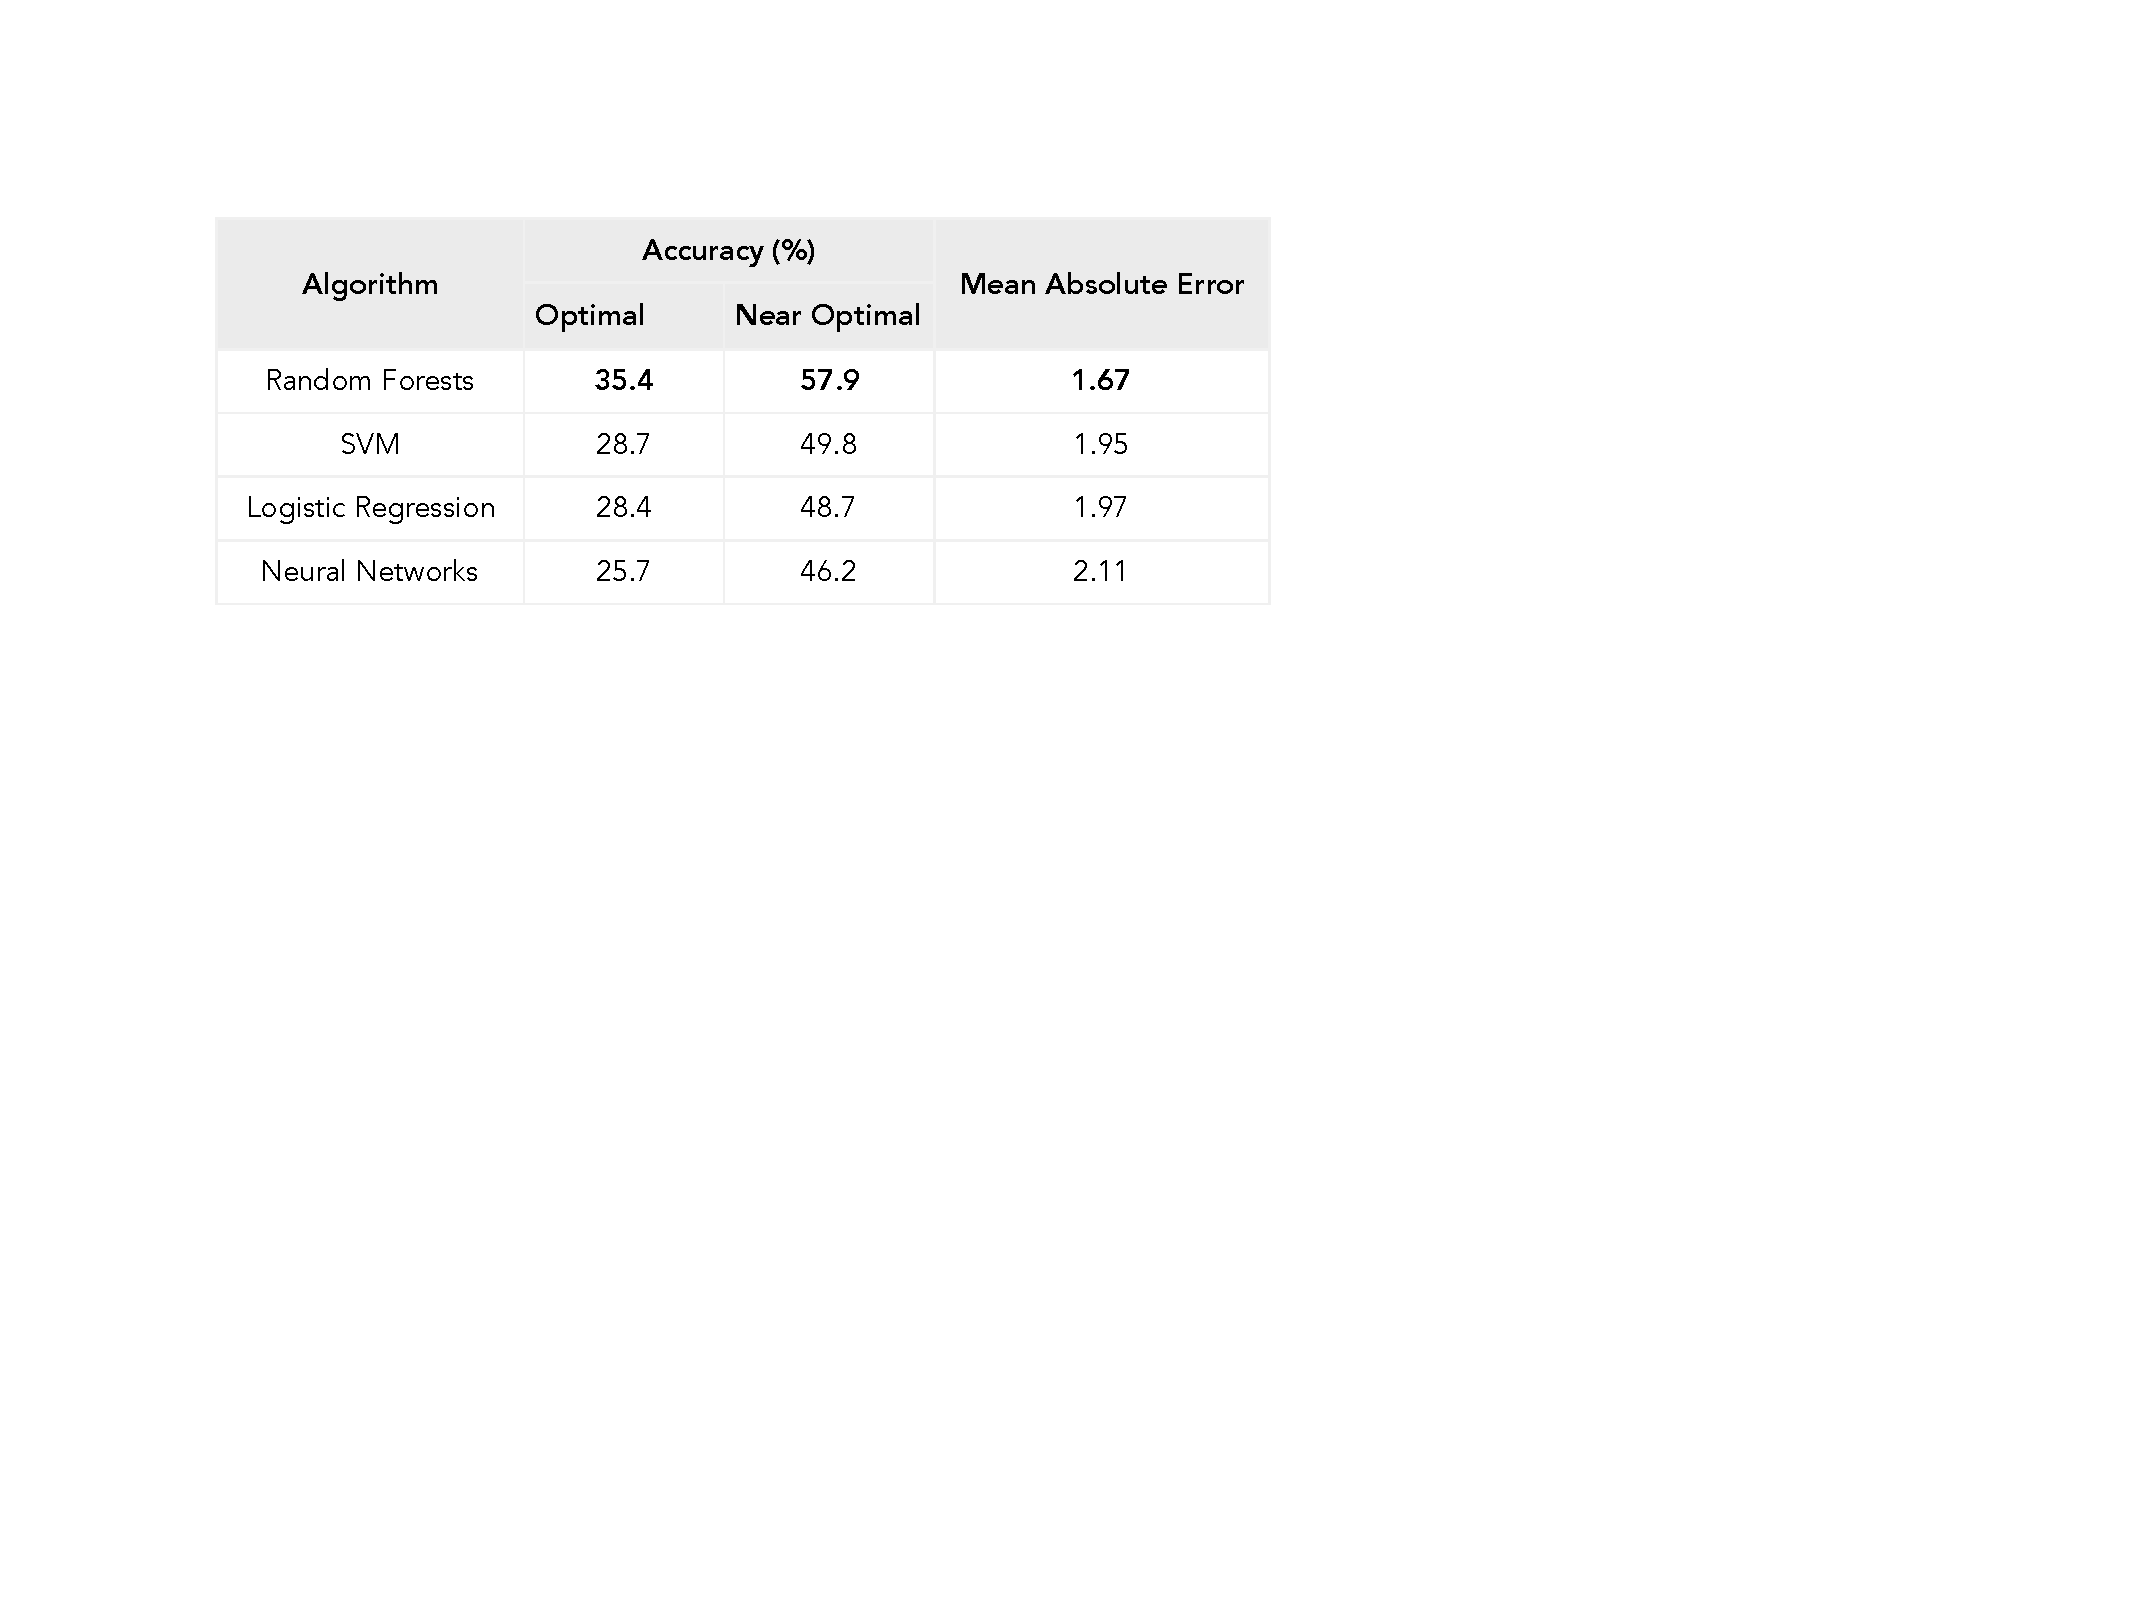
\includegraphics[width=0.\linewidth]{fig/mlApproxResults.pdf}
  \caption{Machine Learning Results}
  \label{fig:mlResults}
\end{figure}

To see how well our algorithm was doing we also decided to map out the distribution of predicted unroll factor vs optimal unroll factor. As can be seen in Figure~\ref{fig:mlPredictions}, our algorithm performed better on lower unroll factors. This can be explained by the slight skew observed in our training data shown in Figure~\ref{fig:trainingHistogram}

\begin{figure}
  \center
  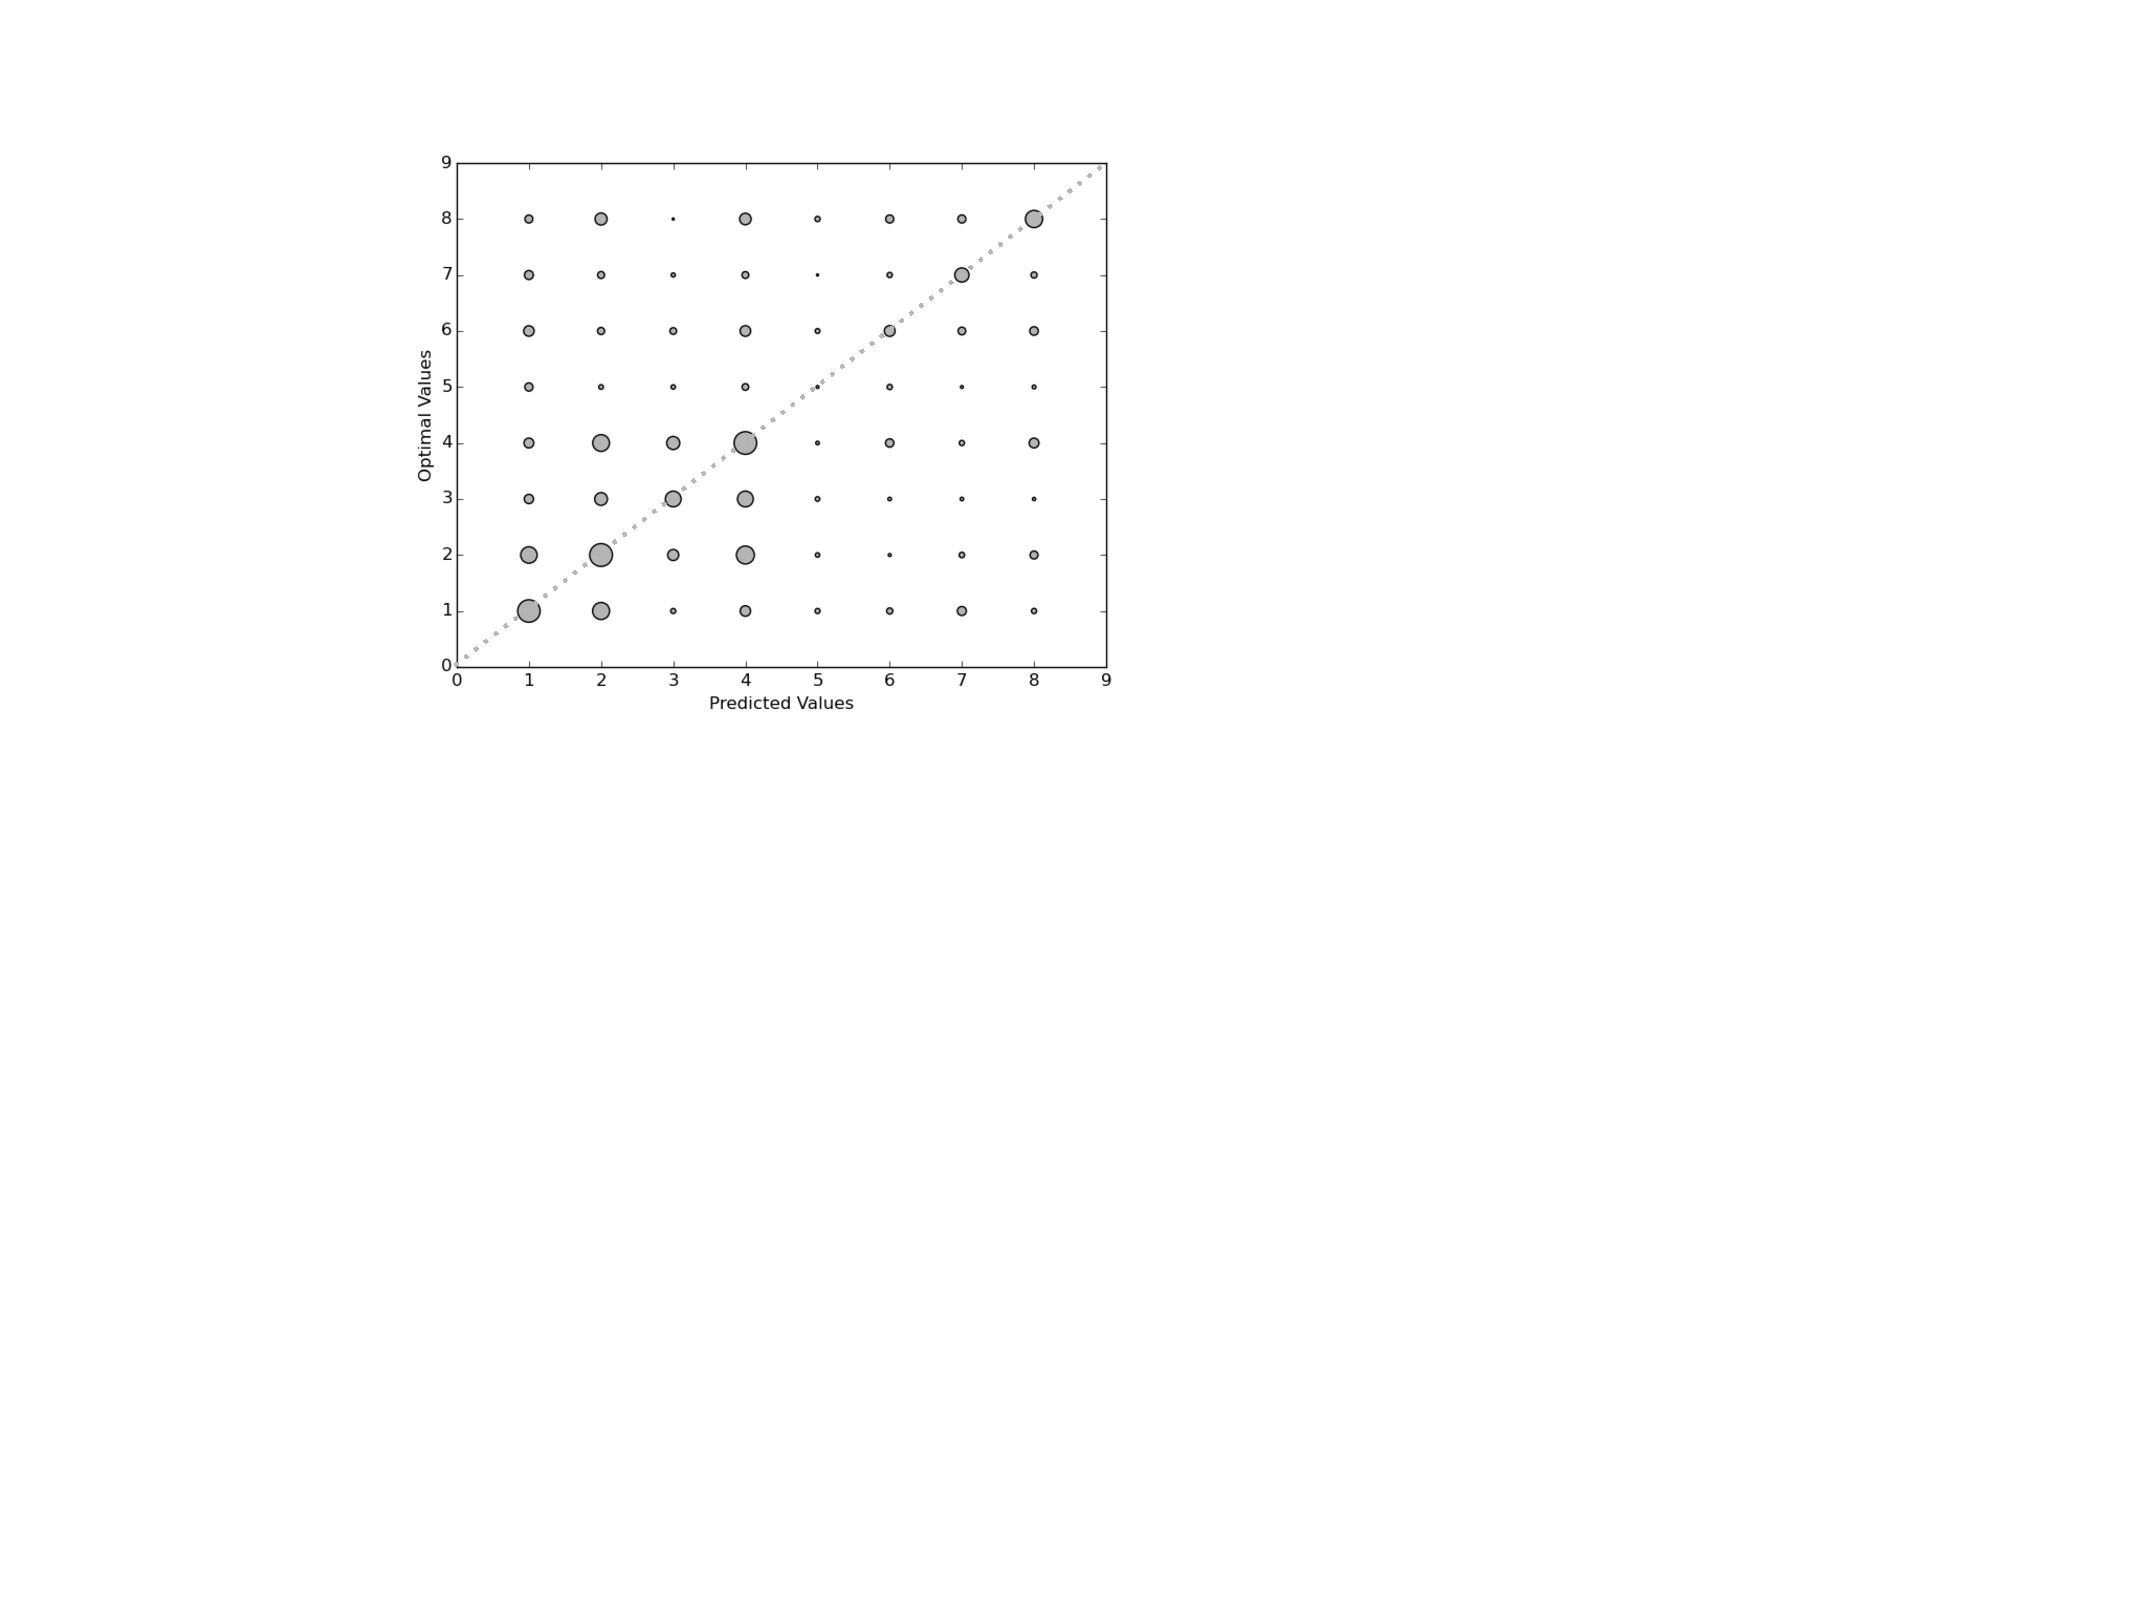
\includegraphics[width=0.90\linewidth]{fig/mlPredictions.pdf}
  \caption{Predictions Distribution}
  \label{fig:mlPredictions}
\end{figure}

% \subsection{Computing the Accuracy}
% \label{subsec:ComputingAccuracy}

% Sort of feel I covered it in the previous sections. 

\section{Experimental Methodology}\label{sec:experimental_methodology}
We developed a random forest trained heuristic for Open Source LLVM Compiler version 3.3. We implemented all the custom passes to unroll and instrument loops and to collect features in LLVM. In addition, we used SPEC 2006 integer and floating point C++ applications to train and test our heuristics. Due to the limited resources available to us, we trained our heuristics on the set of applications having lower number of loops. We trained our heuristics on a training set including 470.lbm, 462.libquantum, 458.sjeng, 456.hmmer, 429.mcf, 401.bzip2, and 445.gobmk applications. Our testing set comprised of the remaining SPEC 2006 applications. We trained and tested our heuristics on Intel Xeon 64-bit 2.2GHz 12-core server with 32KB L1 cache and 256KB L2 cache.


\section{Experimental Results}\label{sec:experimental_results}
In this section we analyze if the predicted unroll factors yield program speedups. We tested our chosen Random Forest classifier on  400.perlbench, 403.gcc, 458.sjeng, 464.h264ref, 471.omnetpp, 473.as.tar and 483.xalancbmk from SPEC CINT 2006. We also tested for speedups on 444.namd, 447.dealll and 450.soplex from SPEC CFP 2006. The test benchmarks are first run through the custom pass for feature extraction. The extracted features are fed to the chosen trained classifier and its output per loop recorded. The test benchmarks are then run through the custom pass for unrolling the loops by the predicted unroll factors In this way we yet again see how well the learned classifier performs on loops not seen before. At this point we run the benchmarks first with no unrolling and with software pipelining disabled. The program run times with no unrolling establish the baseline for us. We then run the benchmarks with loops unrolled by the optimal unroll factors as predicted by our classifier. For comparison, we also run the benchmarks through LLVM's default unroll pass and through a custom pass which unrolls every loop with a randomly chosen unroll factor from 1 through 8. The run times of each test are recorded and the percentage performance improvement achieved in each case is calculated as follows:
\begin{equation}
 \% improvement = \frac{baseline\ run\  time}{test\ run\ time - 1}
\end{equation}

Figure~\ref{fig:cintResults} shows the results on the SPEC CINT 2006 benchmarks. 
While our benchmarks achieve speedups comparable to  LLVM's default heuristics, they almost always beat the random unroll pass.  

Figure~\ref{fig:cfpResults} shows the results on the SPEC CFP 2006 benchmarks. 
\begin{figure}
  \center
  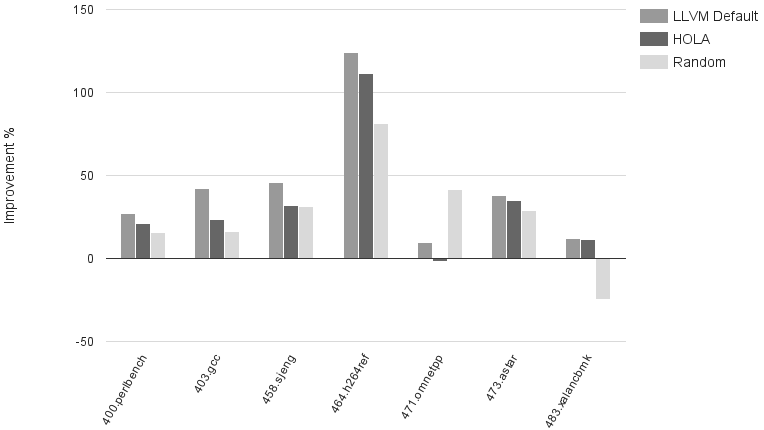
\includegraphics[width=0.90\linewidth]{fig/cint.png}
  \caption{Performance improvement on SPEC CINT 2006 benchmarks}
  \label{fig:cintResults}
\end{figure}
\begin{figure}
  \center
  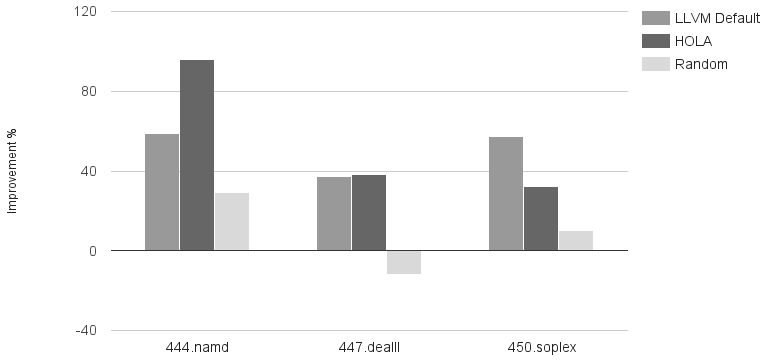
\includegraphics[width=0.90\linewidth]{fig/cfp.png}
  \caption{Performance improvement on SPEC CFP 2006 benchmarks}
  \label{fig:cfpResults}
\end{figure}

HOLA beats LLVM default on all of the CFP benchmarks we tested our predictions on. These results clearly indicate the potential of the machine learning based heuristic to beat the LLVM default heuristic. We achieve an average performance improvement of $33.15 \%$  on the CINT benchmarks and an average improvement of $55.27 \%$. Whereas LLVM default achieves an improvement of $42.57 \%$ on CINT benchmarks and $50.98 \%$ on the CFP benchmarks. 

\section{Discussion}
\label{sec:Discussion}
Compilers are complex tools. It is nearly impossible to know what choices to make based on simple models and assumptions. The scheduler, the register allocator, and the underlying architecture interact in mysterious ways. The only way to truly know what will work is by empirically evaluating decisions. The goal of our research is to use empirical observations to train a compiler to make informed decisions using machine learning based techniques. We believe that machine learning techniques have a strong potential to alter traditional compiler construction techniques. The traditional techniques suffer from some major drawbacks. Consider the case of loop unrolling,  a considerable amount of key information is lost by using heuristics based on thresholding on static features. Also, such compiler heuristics heavily depend upon detailed  knowledge of the system with regards to the implementation of different program transformations, optimizations and the interactions between them. Also, coming up with such heuristics and tuning them efficiently for every platform is anything but pure grunt work. To get rid of this grunt work, we can leverage upon the potential of machine learning based methods to automatically learn and fine tune learned heuristics. This can leave the compiler designers to focus on the actual job of improving the system, build new transformations and optimizations.  However, there are still many issues which need to be addressed before this vision becomes reality. 

Some of the key issues are related to data acquisition and feature engineering. Extracting optimal unroll factors for every loop and generating a large dataset for training can be a  slow process. However, we believe that this was an unsupervised process requiring minimal interference on our part. Another argument is that the compiler writers will have to spend time on feature extraction. Although, most of the features used by us are readily available using LLVM's infrastructure, some of the advanced features might require detailed knowledge of the compiler infrastructure and underlying architecture. However, we believe that features can be made available through special tools within the compiler infrastructure much like various data flow analysis packages are made available. This can cut down on the time required to extract features. Once the data is generated the process of training machine learning classifiers and the online process of prediction is quick. Overall, the effort required is much lesser than the one required for designing heuristics on the part of the compiler writer.  

Another key aspect on which the accuracy of machine learning techniques depends on is the instrumentation process to extract loop labels. The instrumentation to extract loop execution times has its own overhead which can in turn affect the optimal unroll factor introducing noise in the data. One way to counter this would be to use libraries which extract execution times without making use of intrusive system calls. These can be made available within the compiler infrastructure for the greater good of the community.

\section{Related Work}
\label{sec:RelatedWork}
Stephensen et al. use a classifier based on nearest neighbor technique for predicting the loop unroll factors in Open Research Compiler. \cite{stephenson2005predicting} They use Euclidean distance between loop feature vectors as the similarity metric. To generate the loop data they only consider loops that are run for at least 50,000 cycles. The near neighbors algorithm makes prediction based on the labels of points that lie within a specified radius of the new point. They also experiment with an SVM based classifier which performs better than the NN classifier. The NN classifier achieves a classification rate of 62\% while the SVM classifier achieves an accuracy of 65\%.

Monsifrot et al. use a classifier based on ``Boosted'' decision tree
learning to determine which loops to unroll \cite{monsifrot2002machine}.  While the methodology we present in this paper is similar, our work differs in several important ways. Their work only considers binary classification, while our work employ multi-class classification to determine the optimal unroll factor. 

Cavazos et  al. use a machine learning technique namely neuro-evolution, to automatically induce effective method inlining from a set of features deemed useful for inlining \cite{kulkarni2013automatic}. Neuro-evolution is a technique of unsupervised machine learning using neural networks. This methodology can be used in the absence of a good labelled dataset for training purposes. They tested their technique on Maxine VM achieving a speedup of 11\% over the default inlining heuristic in Maxine VM. However, this technique suffers from various drawbacks including long training times and model overfitting.

Davidson et. al. argue that aggressive unrolling leads to significant speedup more often than not\cite{davidson1996aggressive}. This differs from our approach greatly where our method also is capable of doing aggressive unrolling but only when the classification algorithm on extracted features predicts a high unroll factor.

As far as we know, our work is the first of its kind that uses LLVM's infrastructure and Random Forest classifier to learn heuristics for loop unrolling. In our work, we explore all the loops of the program as against related work in the domain which only considers innermost loops or  loops based on their cycle count.

\section{Future Work}
\label{sec:FutureWork}
In the future we would like to explore techniques of less intrusive instrumentation. We also plan on experimenting with instrumenting just the inner loops in a nested loop structure where most of the computation time is spent. In the techniques we explored so far in this work, the predicted unroll factor has a bound which is fixed by the unroll factors we explored during the data generation process. There might be cases when a very high unroll factor for loops might prove to be beneficial. Our technique will not be able to leverage upon this benefit. To counter this, we plan to implement a regression based classifier which can predict optimal unroll factors beyond the range of labels the classifier is trained on.

After an initial evaluation of the results of this work, we infer that increasing the size of the train data set and including additional features involving data flow analysis like ``No. of reaching definitions'', ``Max. dependence height of computations'',  ``No. of memory to memory loop carried dependencies'' etc should lead to an improved accuracy of the classifiers we explored. Additionally, we also plan on exploring more sophisticated machine learning techniques like neural networks which heavily rely upon availability of large training data.

\section{Conclusion}
\label{sec:Conclusion}

In this work, we describe a novel technique for optimizing loop unroll factors using machine learning. We used a Random Forest classifier to make informed decisions about the optimal unroll factors. The optimal unroll factors for the loops in the training data were determined by instrumenting the loops and simulating execution times for various unroll factors. The features for the loops were extracted based on the loop characteristics important to the unroll decision.  

While supervised classification can effectively find good heuristics for multi-class classification, such techniques highly rely on availability of abundant well engineered data for learning. It may take less time to train/tune machine learning algorithms, though can take a much longer time for data acquisition and feature engineering.

Overall, it is a more generalizable approach than platform dependent threshold based heuristics and can automatically learn the optimal parameters. This technique definitely has a huge potential in compiler optimizations like loop unrolling.

\bibliographystyle{IEEEtran}
\begin{scriptsize}
  \bibliography{references}
\end{scriptsize}
\end{document}
